\minitoc

\vfill

\clearpage

\section{\textsc{The general framework}}
    \label{sec::semantic_evaluation::general_framework}

    \subsection{Hierarchization and modularity}
        \label{subsec::semantic_evaluation::general_framework::hierarchization_moderularity}
        As stated previously in subsection~\ref{subsec::introduction::contributions::positioning}, a semantic evaluation implies a categorization of errors affecting building models.
        In the same subsection, we discussed properties that are desired so as to achieve a large scale and automatic semantic evaluation.
        Before delving into details, the implications of such properties on error definitions are examined.

        \subsubsection{\textsc{Generalizability \textit{vs.} exhaustivity compromise}}
            Two conditions are required in the error classification.
            The first one entails the error definitions incongruence with the evaluated urban scenes.
            This implies the proposed error categorization capacity to be generalizable.
            The second is the dissonance between the latter and the input evaluation models.
            This conveys the exhaustivity of the evaluation.\\
            The two notions are condradictory.
            At one hand, every possible error at any level should be taken into account, while, on the other, the categorization has to stay always relevant no matter the origin of those models.
            A compromise have to be reached in the definition of errors between these two properties.
        
        \subsubsection{\textsc{General structure}}
            We porpose a hierarchical structure of the categorization of errors in order to mitigate the last point.
            The more high in the ladder the error is, translates to more generalizability (and less exhaustivity) of the latter.
            At the same level, to avoid having to exhaustively list all possible errors, the identified defects are described modularly based on some predefined independent errors.
            This helps cover a wide range of possible defects while the basic errors are chosen to be as generalizable as possible.
            Hierarchization and modularity are the main ingredients in our proposed flexible framework.\\

            To implement these properties for the error taxonomy, we rely on two criterea for error compilation: the input building model \gls{acr::lod} and the error semantic precision level, named henceforth \texttt{finesse} (cf. Figure~\ref{fig::taxonomy}).
            Different degrees of \texttt{finesse} describe, from coarse to fine, the specificity of defects.
            It corresponds to the error hierarchy levels.
            The \gls{acr::lod} is used on the other hand to differenciate between errors in the same specificity level.
            Multiple errors at the same \texttt{finesse} can indeed affect the same building.
            For instance, topological defects almost always induce (and hence co-occur) with geometrical ones.
            Errors with maximal \texttt{finesse} are called \texttt{atomic} errors.
            \texttt{Atomic} errors are to be intuitively correlated to independent actions needed by an operator or an algorithm so as to correct the model.

    \subsection{\textsc{A general classification of errors}}
        \label{subsec::semantic_evaluation::general_framework::error_classification}
        Herein, based on the previous discussion, a general layout is detailed for building model evaluation.

        At a first level, model qualifiability is studied.
        In fact, aside from formatting issues or geometric inconsistencies~\parencite{ledoux2018val3dity}, other reasons make building models unqualifiable.
        For instance, buildings can be occluded by vegetation and thus cannot be assessed with most of the remote sensing data sources.
        Generally speaking, input models can be impaired by some pathological cases that are outside our evaluation framework.
        In consequence, \texttt{Qualifiable} models are distinguished here from \texttt{Unqualifiable} buildings.
        This first level corresponds to a \texttt{finesse} equal to 0. At the \texttt{finesse} level 1, we predict the correctness of all qualifiable buildings.
        It is the lowest semantization level at which the evaluation of a model is expressed.
        Then, a model is either \texttt{Valid} or \texttt{Erroneous}.
        Most state-of-the-art evaluation methods address errors up to this level.\\
        Model errors are grouped into two families depending on the underlying \gls{acr::lod}.
        The first family of errors \texttt{Building Errors} affects the building in its entirety.
        It corresponds to an accuracy evaluation at \gls{acr::lod}-0 (footprint errors) $\cup$ \gls{acr::lod}-1 (height/geometric error).
        At the next \gls{acr::lod}-2, the family \texttt{Facet Errors} gathers defects that can alter the facet accuracy of fa\c{c}ades or roofs (\gls{acr::lod}-2) as well as superstructures and openings (\gls{acr::lod}-3).\\
        Each family contains \texttt{atomic} errors of maximal \texttt{finesse} equal to 3.
        Although they can co-occur in the same building model and across different families, these errors are semantically independent.
        They represent specific topological or geometric defects.
        Topological errors translate inaccurate structural modeling, while geometric defects raise positioning infidelity.\\

        The general structure is not fixed and can evolve to adapt to more cases.
        In fact, instead of grouping \gls{acr::lod}-2 and \gls{acr::lod}-3 errors, the latter can be made into a different family that can be called \texttt{Superstructure Errors}.
        Due to the lack of sufficient observations, we did not make this choice in order to guaranty the generalizability of the taxonomy.
        Another alternative consists, for instance, in gathering error families by resolution: this will produce a continuum of errors families going from the coarsest level that would correspond to \texttt{Building Errors} to the finest possible one.
        This last option, although offering an exhaustive and potentially generalizable taxonomy, was ruled out since it does not provide a truly semantic description of the errors.
        % For example, an operator that is presented with the error ``segmentation error at resolution 20\%'' would not have any information on 
        Regarding \texttt{finesse}, it is also possible to have additional levels.
        The maximal level of 3 was chosen in order to preserve the generalizability of the taxonomy, since the more specific the error categorization is, the more observations we need to define the corresponding errors.

        \begin{figure}
            \begin{center}
                \includestandalone[mode=buildnew, width=\textwidth]{figures/taxonomy_tree}
                \caption{
                    \label{fig::taxonomy} 
                    The proposed taxonomy structure.
                    In our case of very high resolution overhead image modeling, only two family errors are depicted.
                    At \texttt{finesse} level 2, hierarchization is possible: the \textbf{exclusivity} parameter can thus act.
                    However, it is not the case at the \texttt{atomic} errors level since they are independent.
                }
            \end{center}
        \end{figure}

\section{\textsc{Application to the geospatial overhead case}}
    \label{sec::semantic_evaluation::overhead}
    Our observations were based on large datasets of \gls{acr::3d} models of buildings reconstructed automatically using \gls{acr::vhr} geospatial images or, if available, \gls{acr::lidar} point clouds.
    We apply the framework introduced in the previous subsection to our special case.
    To do so, we will define the \texttt{atomic} errors before discussing their propoerties.

    \subsection{\textsc{Atomic error definitions}}
        \label{subsec::semantic_evaluation::overhead::atomic}
        In the template structure presented in section~\ref{subsec::semantic_evaluation::general_framework::error_classification}, were left out the \texttt{atomic} error definitions.
        Indeed, since they represent the most specific level, their choice is critical to guaranty both the exhaustivity and generalizability we are hoping for.
        We conducted a thourough inspection of all defects that we detected in our datasets and came up with the following definitions (\textit{cf.} Figures~\ref{fig::taxonomy}).
        \subsubsection{\texttt{Building errors} \textsc{family}}
            Herein are presented the \texttt{atomic} errors regarding the \gls{acr::lod}-0 and \gls{acr::lod}-1 ascpects.

            \paragraph{\texttt{\acrlong*{acr::bus}}}
                \begin{figure}
                    \centering
                    \ffigbox[\FBwidth]{
                        \begin{subfloatrow}[2]
                            \ffigbox[\FBwidth]{
                                \includegraphics[width=.45\textwidth]{example-image}
                            }{
                                \label{subfig::bus_3d}
                                \caption{
                                    Depiction of the a case where two building that are reconstructed as one.
                                }
                            }
                            \ffigbox[\FBwidth]{
                                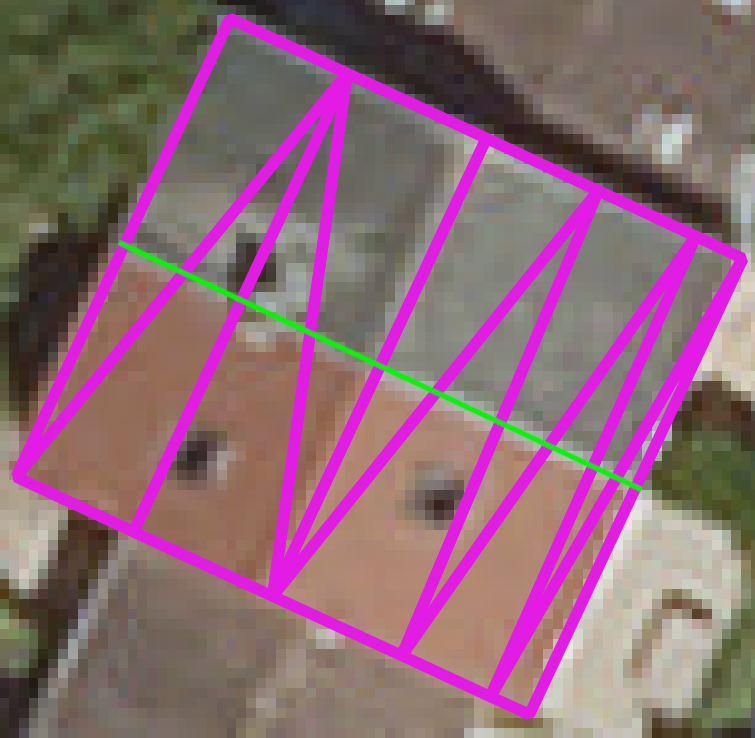
\includegraphics[width=.45\textwidth]{images/errors/building/under_segmentation}
                            }{
                                \label{subfig::bus_2d}
                                \caption{
                                    Nadir projection of the erroneous building superposed on the corresponding orthoimage.
                                    We can recognize, based on the color differences of roof tiles, the existance of two buildings instead of one.
                                }
                            }
                        \end{subfloatrow}
                    }{
                        \caption{
                            \label{fig::bus}
                            Illustration of a \gls{acr::bus} error.
                        }
                    }
                \end{figure}

                \gls{acr::bus} corresponds to the case where two or more buildings are modeled as one.
                In Figure~\ref{fig::bus}, two distinct buildings were identified as one building, eventhough they can be visually distinguished.

                This error is very common and results from a faulty footprint of the building.
                The latter is either retrieved automatically during the modeling~\parencite{lafarge2012creating}, or is provided as input~\parencite{durupt2006automatic}.
                The first case is the most error inducing as it relies on extrinsic large scale remote sensing data that are devoid of semantics.
                The second is expected to be more close to the reality, but can be unsuitable if outdated.

            \paragraph{\texttt{\acrlong*{acr::bos}}}
                \begin{figure}
                    \centering
                    \ffigbox[\FBwidth]{
                        \begin{subfloatrow}[2]
                            \ffigbox[\FBwidth]{
                                \includegraphics[width=.45\textwidth]{example-image}
                            }{
                                \label{subfig::bos_3d}
                                \caption{
                                    Depiction of the a case where two building that are reconstructed as one.
                                }
                            }
                            \ffigbox[\FBwidth]{
                                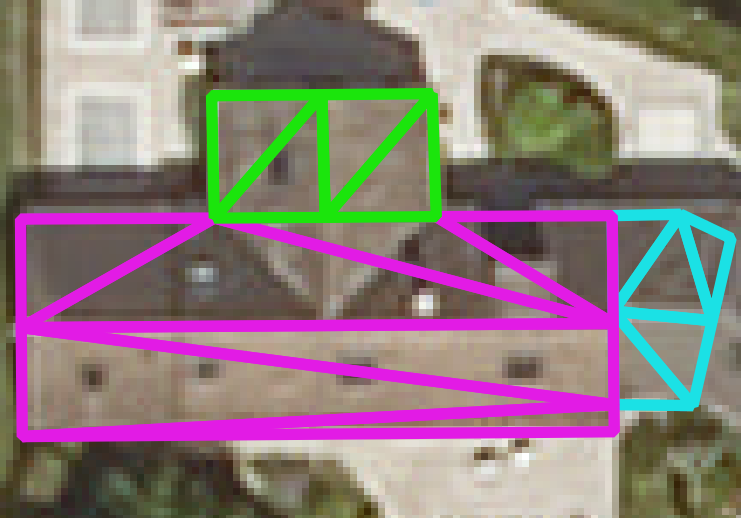
\includegraphics[width=.45\textwidth]{images/errors/building/over_segmentation}
                            }{
                                \label{subfig::bos_2d}
                                \caption{
                                    Nadir projection of the erroneous building superposed on the corresponding orthoimage.
                                    We can recognize, based on the color differences of roof tiles, the existance of two buildings instead of one.
                                }
                            }
                        \end{subfloatrow}
                    }{
                        \caption{
                            \label{fig::bos}
                            Illustration of a \gls{acr::bos} error.
                        }
                    }
                \end{figure}

                \gls{acr::bos} corresponds to the case where one building is subdivided into two or more buildings.
                This is the opposite of the previous situation.
                Figure~\ref{fig::bos} shows a single building that, when modelled, was subdivided into three parts.

            \paragraph{\texttt{\acrlong*{acr::bib}}}
                \begin{figure}
                    \centering
                    \ffigbox[\FBwidth]{
                        \begin{subfloatrow}[2]
                            \ffigbox[\FBwidth]{
                                \includegraphics[width=.45\textwidth]{example-image}
                            }{
                                \label{subfig::bib_3d}
                                \caption{\gls{acr::3d} depiction of the error.}
                            }
                            \ffigbox[\FBwidth]{
                                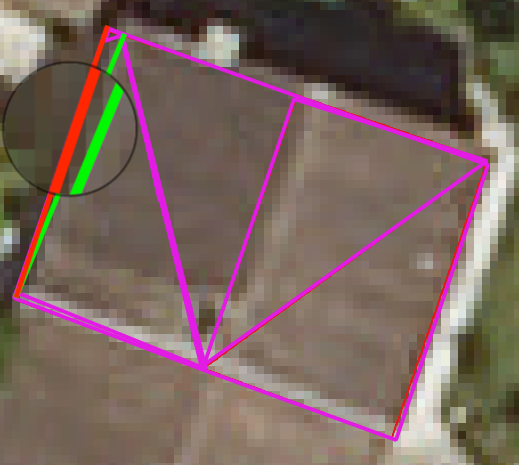
\includegraphics[width=.45\textwidth]{images/errors/building/border}
                            }{
                                \label{subfig::bib_2d}
                                \caption{
                                    Nadir projection of the erroneous building superposed on the corresponding orthoimage.
                                }
                            }
                        \end{subfloatrow}
                    }{
                        \caption{
                            \label{fig::bib}
                            Illustration of a \gls{acr::bib} error.
                        }
                    }
                \end{figure}

                \gls{acr::bib} corresponds to the case where at least one building footprint border is incorrectly located.
                A sample is shown in Figure~\ref{fig::bib}.

            \paragraph{\texttt{\acrlong*{acr::bit}}}
                \begin{figure}
                    \centering
                    \ffigbox[\FBwidth]{
                        \begin{subfloatrow}[2]
                            \ffigbox[\FBwidth]{
                                \includegraphics[width=.45\textwidth]{example-image}
                            }{
                                \label{subfig::bit_3d}
                                \caption{\gls{acr::3d} depiction of the error.}
                            }
                            \ffigbox[\FBwidth]{
                                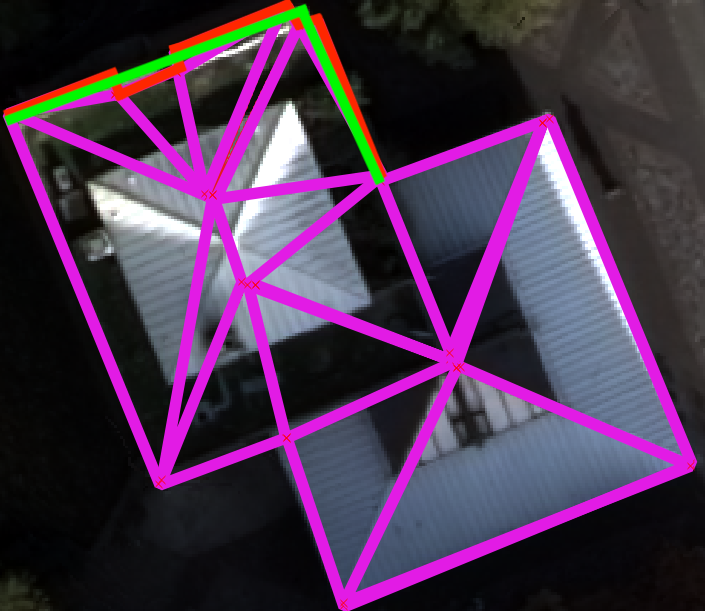
\includegraphics[width=.45\textwidth]{images/errors/building/topology}
                            }{
                                \label{subfig::bit_2d}
                                \caption{
                                    Nadir projection of the erroneous building superposed on the corresponding orthoimage.
                                }
                            }
                        \end{subfloatrow}
                    }{
                        \caption{
                            \label{fig::bit}
                            Illustration of a \gls{acr::bit} error.
                        }
                    }
                \end{figure}

                \gls{acr::bit} corresponds to the case where the building footprint suffers from topological defects as missing inner courts or wrong primitive fitting (for instance, a circular footprint approximated by a polygon).
                In Figure~\ref{fig::bit}, we illustrate how the footprint morphology can be erroneous.
                This error, as the earlier ones, result either from defective building identification process, or from an outdated cadastral map.

            \paragraph{\texttt{\acrlong*{acr::big}}}
                \gls{acr::big} corresponds to the case of inaccurate building geometric estimation.
                In case \textbf{\gls{acr::elod}} > \gls{acr::lod}-0 $\cup$ \gls{acr::lod}-1, this error is not reported as it becomes redundant with below delineated errors.
            
        \subsubsection{\texttt{Facet errors} \textsc{family}}
            In this sub-subsection, \gls{acr::lod}-2 and \gls{acr::lod}-3 corresponding \texttt{atomic} errors are presented.

            \paragraph{\texttt{\acrlong*{acr::fus}}}
                \begin{figure}
                    \centering
                    \ffigbox[\FBwidth]{
                        \begin{subfloatrow}[2]
                            \ffigbox[\FBwidth]{
                                \includegraphics[width=.45\textwidth]{example-image}
                            }{
                                \label{subfig::fus_3d}
                                \caption{
                                    Depiction of the a case where two building that are reconstructed as one.
                                }
                            }
                            \ffigbox[\FBwidth]{
                                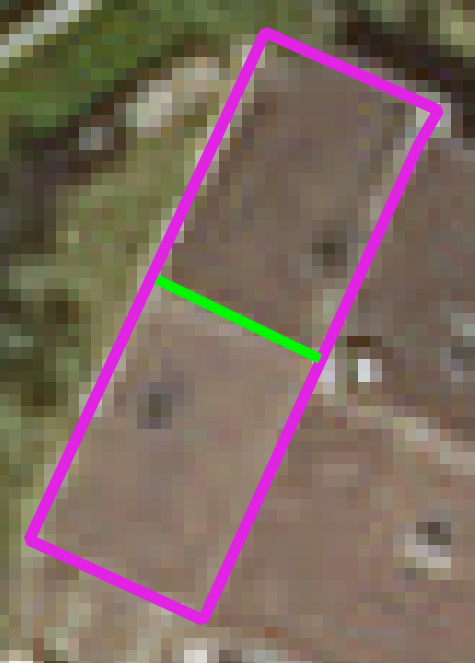
\includegraphics[width=.45\textwidth, angle=270]{images/errors/facet/under_segmentation}
                            }{
                                \label{subfig::fus_2d}
                                \caption{
                                    Nadir projection of the erroneous building superposed on the corresponding orthoimage.
                                    We can recognize, based on the color differences of roof tiles, the existance of two buildings instead of one.
                                }
                            }
                        \end{subfloatrow}
                    }{
                        \caption{
                            \label{fig::fus}
                            Illustration of a \gls{acr::fus} error.
                        }
                    }
                \end{figure}

                \gls{acr::fus} corresponds to the case where one facet is subdivided into two or more facets.
                Refer to Figure~\ref{fig::fus} for an example.

                This error is very common and results from a faulty footprint of the building.
                The latter is either retrieved automatically during the modeling~\parencite{lafarge2012creating}, or is provided as input~\parencite{durupt2006automatic}.
                The first case is the most error inducing as it relies on extrinsic large scale remote sensing data that are devoid of semantics.
                The second is expected to be more close to the reality, but can be unsuitable if outdated.

            \paragraph{\texttt{\acrlong*{acr::fos}}}
                \begin{figure}
                    \centering
                    \ffigbox[\FBwidth]{
                        \begin{subfloatrow}[2]
                            \ffigbox[\FBwidth]{
                                \includegraphics[width=.45\textwidth]{example-image}
                            }{
                                \label{subfig::fos_3d}
                                \caption{\gls{acr::3d} depiction of the error.}
                            }
                            \ffigbox[\FBwidth]{
                                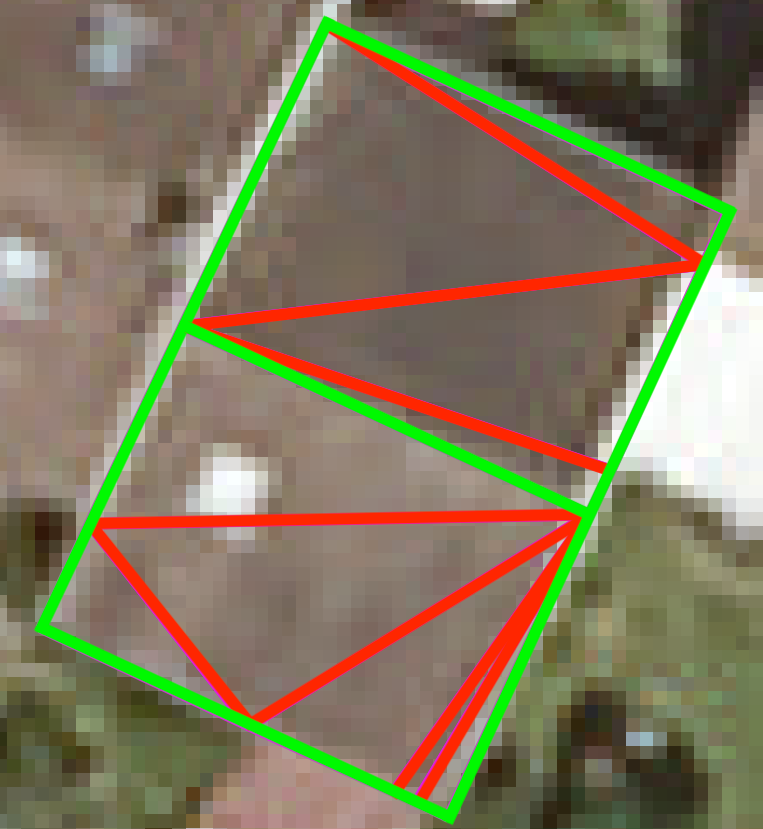
\includegraphics[width=.45\textwidth, angle=270]{images/errors/facet/over_segmentation}
                            }{
                                \label{subfig::fos_2d}
                                \caption{
                                    Nadir projection of the erroneous building superposed on the corresponding orthoimage.
                                }
                            }
                        \end{subfloatrow}
                    }{
                        \caption{
                            \label{fig::fos}
                            Illustration of a \gls{acr::fos} error.
                        }
                    }
                \end{figure}

                \gls{acr::fos} corresponds to the case where two or more facets are modeled as one, as illustrated in Figure~\ref{fig::fos}.

            \paragraph{\texttt{\acrlong*{acr::fib}}}
                \begin{figure}
                    \centering
                    \ffigbox[\FBwidth]{
                        \begin{subfloatrow}[2]
                            \ffigbox[\FBwidth]{
                                \includegraphics[width=.45\textwidth]{example-image}
                            }{
                                \label{subfig::fib_3d}
                                \caption{\gls{acr::3d} depiction of the error.}
                            }
                            \ffigbox[\FBwidth]{
                                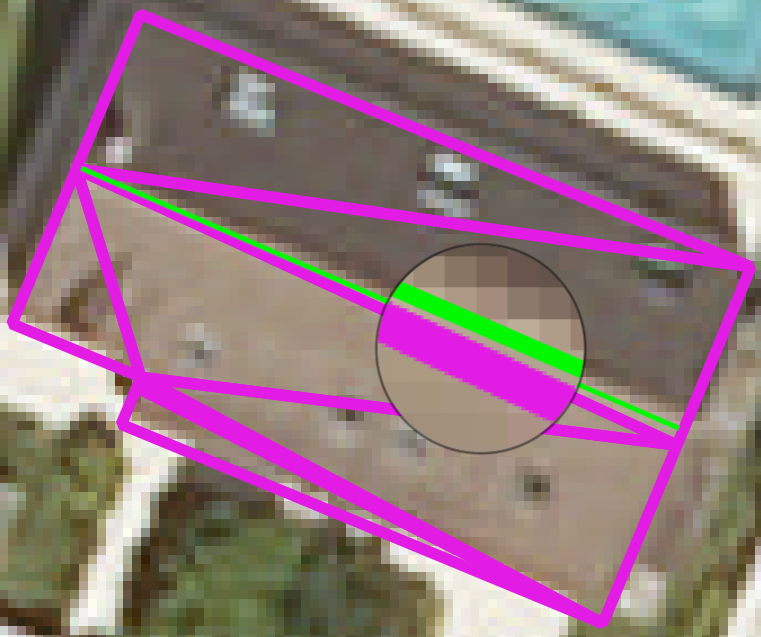
\includegraphics[width=.45\textwidth]{images/errors/facet/border}
                            }{
                                \label{subfig::fib_2d}
                                \caption{
                                    Nadir projection of the erroneous building superposed on the corresponding orthoimage.
                                }
                            }
                        \end{subfloatrow}
                    }{
                        \caption{
                            \label{fig::fib}
                            Illustration of a \gls{acr::fib} error.
                        }
                    }
                \end{figure}

                \gls{acr::fib} corresponds to the case where at least one facet border is incorrectly located.
                As en example, Figure~\ref{fig::fib} shows that the central edge that links the two main roof sides does not correspond to the one on the image position.

            \paragraph{\texttt{\acrlong*{acr::fit}}}
                \begin{figure}
                    \centering
                    \ffigbox[\FBwidth]{
                        \begin{subfloatrow}[2]
                            \ffigbox[\FBwidth]{
                                \includegraphics[width=.45\textwidth]{example-image}
                            }{
                                \label{subfig::fit_3d}
                                \caption{\gls{acr::3d} depiction of the error.}
                            }
                            \ffigbox[\FBwidth]{
                                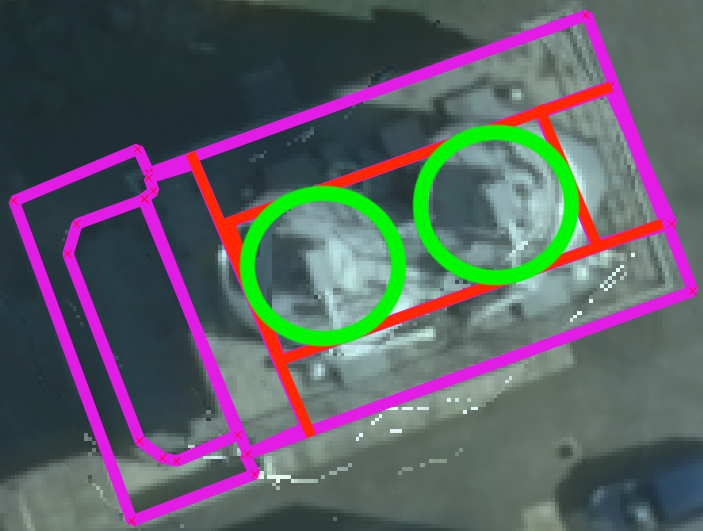
\includegraphics[width=.45\textwidth]{images/errors/facet/topology}
                            }{
                                \label{subfig::fit_2d}
                                \caption{
                                    Nadir projection of the erroneous building superposed on the corresponding orthoimage.
                                }
                            }
                        \end{subfloatrow}
                    }{
                        \caption{
                            \label{fig::fit}
                            Illustration of a \gls{acr::fit} error.
                        }
                    }
                \end{figure}

                \gls{acr::fit} corresponds to the case where the facet suffers from topological defects such as wrong primitive fitting (for example, a dome approximated by planar polygons).
                In Figure~\ref{fig::fit}, we can observe how two cylindrical towers were reconstructed as a rectangular parallelepiped.

            \paragraph{\texttt{\acrlong*{acr::fig}}}
                \begin{figure}
                    \centering
                    \ffigbox[\FBwidth]{
                        \begin{subfloatrow}[2]
                            \ffigbox[\FBwidth]{
                                \includegraphics[width=.45\textwidth]{example-image}
                            }{
                                \label{subfig::fig_3d}
                                \caption{\gls{acr::3d} depiction of the error.}
                            }
                            \ffigbox[\FBwidth]{
                                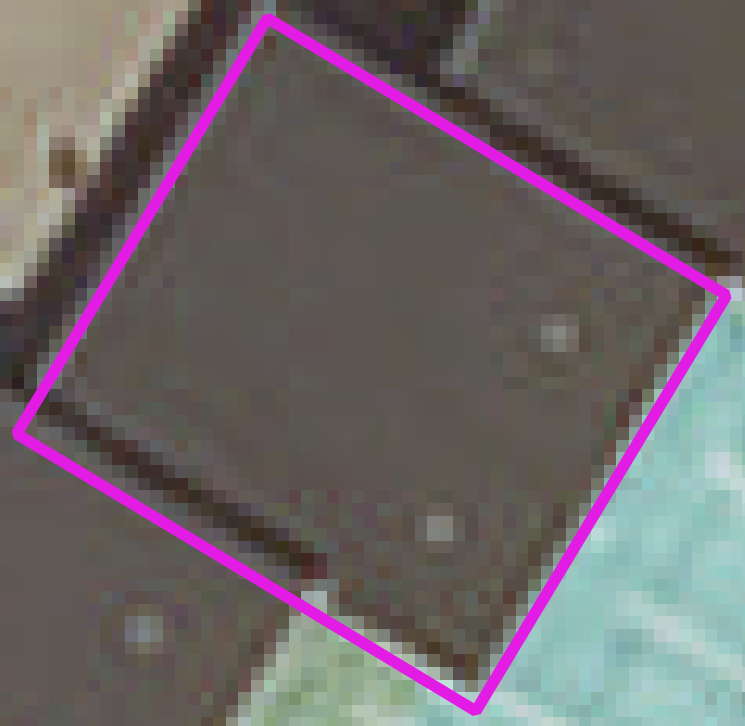
\includegraphics[width=.45\textwidth]{images/errors/facet/geometry}
                            }{
                                \label{subfig::fig_2d}
                                \caption{
                                    Nadir projection of the erroneous building superposed on the corresponding orthoimage.
                                }
                            }
                        \end{subfloatrow}
                    }{
                        \caption{
                            \label{fig::fig}
                            Illustration of a \gls{acr::fig} error.
                        }
                    }
                \end{figure}

                \gls{acr::fig} corresponds to the case of inaccurate facet geometric estimation :\textit{e.g.}, wrong height or inaccurate slope.
                The latter is depicted in Figure~\ref{fig::fig}\footnote{
                    There is a problem of slope. The model corresponds to a flat roof whereas in reality the slope is \textit{ca.} \SI{25}{\degree}.
                    The error could only be shown if we provided the height residual.
                    However, for the sake of homogeneity, we only provided orthoimages as background.
                    It motivates also the need for a height-based modality.
                    All these errors stem either from the modeling approach, or from the poor spatial resolution of the input data (DSM or point cloud)
                }.

    \subsection{\textsc{Discussion}}
        \label{subsec::semantic_evaluation::overhead::discussion}
        These errors can be related to state-of-the-art labels.
        For instance, ``Missing Node'' (\textit{resp.} ``False Node'', ``Missing Edge'' and ``False Edge'') in~\citet{xiong2014graph} correspond to, or are included in, the topological \textit{atomic} errors from the \textit{Facet Errors} family: \texttt{FUS} (\textit{resp.} \texttt{FOS}, \texttt{FIT}, and \texttt{FIT}).
        The difference is that we distinguish flaws that can affect superstructure facets (\gls*{acr::lod}-3) from the ones that impair building facets (\gls*{acr::lod}-2).
        The taxonomy developed by~\citet{Michelin2013}\reviewed{, on the other hand, is closer to ours}.
        In fact, while footprint errors is reshuffled into \textit{Building Errors} as \texttt{BIB} (``erroneous outline'' and ``imprecise footprint'') and \texttt{BIT} (``missing inner court'') , intrinsic reconstruction errors (``over-segmentation'', ``under segmentation'', ``inexact roof'' and ``Z translation'') can be re-adapted into both family errors.
        Finally, ``vegetation occlusion'' and `` non existing'' are gathered into the \textit{unqualifiable} label at \textit{finesse} level 0.~\citet{boudet2006supervised}, however, studied the acceptability of a model in a whole.
        Their taxonomy cannot directly fit with our labels.
        The acceptability dimension can be incorporated into our framework by attributing an confidence score to each error: for example, a prediction probability.        

\section{\textsc{Parametric label extraction}}
        \label{sec::semantic_evaluation::label_extraction}
    At evaluation time, three parameters play a role in determining which error labels to consider.
    The first is the \textbf{\gls{acr::elod}}. Every reconstruction method targets a certain set of \glspl{acr::lod}.
    In consequence, when assessing a reconstruction, a \gls{acr::lod} must be specified. At a given \gls{acr::elod}, all error families involving higher orders will be ignored.
    Depending on the target of the qualification process, a \textbf{finesse} level might be preferred.
    This second evaluation parameter specifies the appropriate semantic level at which errors will be reported.
    The last one is error \textbf{exclusivity}. It conveys family error hierarchy. Errors of a given \gls{acr::lod}$ = l$ family are prioritized over ones with higher \gls{acr::lod}$ > l$.

    \subsection{\textsc{Evaluation parameters}}
    \subsection{\textsc{Evaluation labels}}
